%! TEX program = xelatex
%! TEX encoding = UTF-8 Unicode

\documentclass[engineeringmaster]{hquThesis}
\usepackage{lineno}
\usepackage{amsmath,amsfonts,amssymb,textcomp,ulem}
\usepackage{booktabs,multirow,tabularx,float}
\usepackage{listings}




\hypersetup{colorlinks=true,linkcolor=black,citecolor=black}
\begin{document}
\makecover
% NOTE: 正式文档请取消下面两行注释
% {
    \begin{center}
        \sffamily\fontsize{16pt}{25pt}\selectfont 学\hspace{8pt}位\hspace{8pt}论\hspace{8pt}文\hspace{8pt}答\hspace{8pt}辩\hspace{8pt}委\hspace{8pt}员\hspace{8pt}会\hspace{8pt}决\hspace{8pt}议
    \end{center}
} \vspace{32pt}
{
    \fontsize{14pt}{26pt}\selectfont
    \noindent\hspace{28pt}\rmfamily 根据《中华人民共和国学位条例》、《中华人民共和国学位条例暂行实 施办法》、《华侨大学学位授予工作细则》及《华侨大学研究生学位论文质 量监控与评阅答辩的管理规定》的规定,学位论文答辩委员会经充分交换意 见,对论文做出评价,并以无记名投票方式进行表决,同意该同学通过\degree 学位论文答辩,同意授予\degree 学位。\par
    \vspace{192pt}
    \noindent\flushright 答辩委员会(主席签字):\underline{\hspace{156pt}}\vspace{14pt} \par
    \noindent\flushright 答辩时间:\underline{\hspace{60pt}}年\underline{\hspace{25pt}}月\underline{\hspace{25pt}}日 \par
}

% \noindent\fbox{%
    \parbox{14.3cm}{
    \vspace{24pt}\begin{center}\sffamily\fontsize{16pt}{\baselineskip}\selectfont 学位论文独创性声明\end{center}\vspace{18pt}
    \hspace{28pt}\declarationfont\fontsize{14pt}{28pt}\selectfont
    本人声明兹呈交的学位论文是本人在导师指导下完成的研究成果。论文写作中不包含其他人已经发表或撰写过的研究内容,如参考他人或集体的科研成果,均在论文中以明确的方式说明。本人依法享有和承担由此论文所产生的权利和责任。\par
    \vspace{28pt}\hspace{28pt} 论文作者签名:\underline{\hspace{112pt}}\hspace{7pt}签名日期:\underline{\hspace{77pt}}\par\vspace{7pt}
    }%
}
\par
\vspace{44pt}
\noindent\framebox[\linewidth]{
    \parbox{14.3cm}{
    \vspace{24pt}\begin{center}\sffamily\fontsize{16pt}{\baselineskip}\selectfont 学位论文版权使用授权声明\par\end{center}\vspace{18pt}
    \hspace{28pt}\declarationfont\fontsize{14pt}{28pt}\selectfont 
    本人同意授权华侨大学有权保留并向国家机关或机构送交学位论文的复印件和电子版,允许学位论文被查阅和借阅。本人授权华侨大学可以将本学位论文的全部内容或部分内容编入有关数据库进行检索,可以采用影印、缩印或扫描等复制手段保存和汇编本学位论文。\par\vspace{28pt}
    \hspace{28pt}论文作者签名:\underline{\hspace{84pt}}\hspace{7pt}指导老师签名:\underline{\hspace{84pt}}\par
    \hspace{28pt}签\hspace{7pt}名\hspace{7pt}日\hspace{7pt}期:\underline{\hspace{91pt}}\hspace{7pt}签\hspace{7pt}名\hspace{7pt}日\hspace{7pt}期:\underline{\hspace{91pt}}\par\vspace{7pt}
    }
}


\frontmatter{
    
\begin{abstract}
自锁问题是有限元分析中的一类常见数值问题,主要表现为在模拟某些特定物理现象时,数值解因过度约束而丧失精度或收敛性。
常见的自锁问题包括以下两类:体积自锁:在模拟不可压缩材料时,由于体积应变能的过度约束,导致数值解出现刚化现象,无法准确描述材料的变形特性;剪切自锁:在模拟中厚板结构时,由于剪切应变能的过度约束,导致数值解无法准确反映结构的实际变形行为。
混合有限元法是解决自锁问题的常用方法,通过引入额外的场变量(如压力场)来减少过度约束。
例如,在不可压问题中,使用位移--压力混合离散可以有效缓解体积自锁现象。
然而,混合有限元法必须满足LBB稳定性条件,才能保证数值解的稳定性,在一定情况下也可能会产生压力振荡现象。因此,选择合适的变量间约束比至关重要。
尽管混合有限元法常用于解决自锁问题,但并非所有混合离散方案都满足LBB稳定性条件,而已知的满足LBB稳定性条件的混合离散方案常常表现出过度约束的状态。
无网格法具有不依赖于几何拓扑关系的高阶光滑形函数,能够任意的布置节点,特别适用于变量间的混合离散过程。通过结合无网格法与混合有限元法,可以有效解决传统方法中的问题。

本文针对传统混合离散方案存在的问题,提出了一种有限元无网格混合离散分析方法。
并在该方法的基础上,研究了体积不可压问题和中厚板剪切自锁问题中离散节点分布与LBB稳定性条件之间的关系,建立了考虑最优约束比的LBB稳定性条件验证方法,从而确定免自锁的最优约束比范围。
依托再生核无网格法理论框架,通过调整约束比,生成了一种免自锁且满足LBB稳定性条件的有限元无网格混合离散方案。
最后,通过体积不可压问题和中厚板问题的系列经典算例,验证了所提LBB稳定性条件验证方法的正确性,以及有限元无网格混合离散方案的计算精度和稳定性。

\end{abstract}
\keywords{自锁问题;混合离散;最优约束比;LBB稳定性条件;无网格法}

\begin{abstractEn}
Locking problems are a common class of numerical issues in finite element analysis, primarily manifested as a loss of accuracy or convergence in numerical solutions due to excessive constraints when simulating specific physical phenomena. 
Typical locking problems include two categories: volumetric locking, where numerical solutions exhibit artificial stiffening due to over-constrained volumetric strain energy in modeling incompressible materials, and shear locking, where numerical solutions fail to accurately reflect the deformation behavior of moderately thick plate structures due to over-constrained shear strain energy. 
The mixed finite element method is widely used to address locking problems by introducing additional field variables (e.g., pressure fields) to relax excessive constraints. For instance, displacement-pressure mixed discretization effectively mitigates volumetric locking in incompressible problems. 
However, the mixed finite element method must satisfy the LBB (Ladyzhenskaya-Babuška-Brezzi) stability conditions to ensure numerical stability, and pressure oscillations may still occur under certain circumstances. 
Therefore, selecting an appropriate constraint ratio between variables is critical. Although the mixed finite element method is commonly employed to resolve locking problems, not all mixed discretization schemes satisfy the LBB stability conditions. Even known LBB-compliant schemes often exhibit over-constrained states.
Meshfree methods, characterized by high-order smooth shape functions independent of geometric topology and flexible node arrangement, are particularly suitable for mixed discretization processes involving multiple variables. By integrating meshfree methods with the mixed finite element approach, traditional limitations can be effectively addressed.

This study proposes a finite element-meshfree hybrid discretization method to tackle the shortcomings of conventional mixed discretization schemes. 
Building on this method, the relationship between discrete node distributions and LBB stability conditions is systematically investigated for both incompressible problems and moderately thick plate shear locking problems.
A verification framework for LBB stability conditions incorporating an optimal constraint ratio is established to determine the optimal constraint range for locking-free solutions. 
Leveraging the theoretical framework of the reproducing kernel meshfree method, a locking-free hybrid discretization scheme satisfying LBB stability conditions is developed by adjusting the constraint ratio. 
Finally, a series of benchmark cases for incompressible problems and moderately thick plate problems validate the correctness of the proposed LBB stability verification framework and demonstrate the computational accuracy and stability of the finite element-meshfree hybrid discretization scheme.

\end{abstractEn}
\keywordsEn{Locking problems; Mixed discretization;  Optimal constraint ratio;LBB stability conditions; Meshfree method}

    \tableofcontents
}

\mainmatter
\chapter{前期准备}
\section{封面关键字设置}
\section{Git相关}
\begin{enumerate}
    \item 通过fork建仓,具体步骤可参考\href{https://docs.github.com/en/repositories/creating-and-managing-repositories/creating-a-template-repository}{这里}。
    \item 设置 .gitignore 文件(已配置)。
\item 设置临时文件(.aux、.bbl等)和编译文件(.pdf)位置,具体可参考\href{https://github.com/James-Yu/LaTeX-Workshop/wiki/Compile#latex-tools}{LaTeX-Workshop帮助文档}(设置\%TMPDIR\%、\%OUTDIR\%)。
\end{enumerate}

\section{VS code配置}
\subsection*{配置Latex}
\href{https://github.com/James-Yu/LaTeX-Workshop/wiki/Compile#latex-tools}{LaTeX-Workshop配置}
\subsection*{LaTeX workshop: }

正向搜索(forward research)从代码处定位至PDF文档处:Ctrl+alt+j

反向搜索(inverse research)从PDF文档准确定位至LaTeX代码处:Ctrl+鼠标左键

正反向搜索具体教程可参考\href{https://github.com/James-Yu/LaTeX-Workshop/wiki/View#synctex}{这里}。
\subsection*{Git Graph}
点击左侧源代码管理插件-点击左上角View Git Graph(git log)-查看修改记录

\subsection*{Todo Tree}
帮助管理项目中的TODO注释和其他标记,\href{https://blog.csdn.net/m0_37586991/article/details/104239568}{Todo Tree安装步骤}。

\subsection*{Zotero LaTeX}
Zotero管理参考文献
\section{文件、label 命名规则}
Latex路径中文件只允许以英文命名

\subsection*{公式}
\begin{lstlisting}[language=TeX]
    \label{CH_name}{formula_name}
\end{lstlisting}

\subsection*{图}
\begin{lstlisting}
    \label{CH_name}{fig_name}
\end{lstlisting}

\subsection*{表}
\begin{lstlisting}
    \label{CH_name}{table_name}
\end{lstlisting}


\chapter{图表设置}
\subsection*{单张}
\begin{figure}[H]
    \centering
    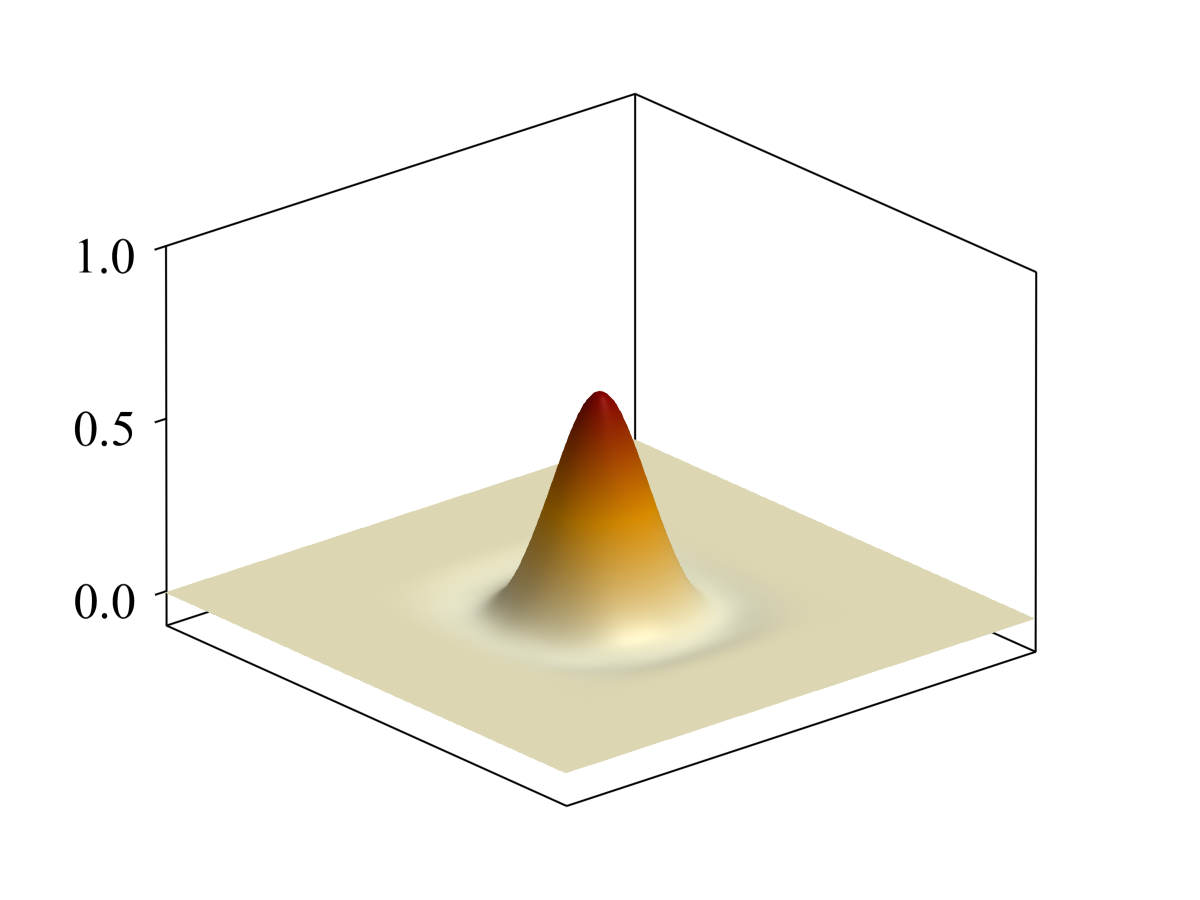
\includegraphics[scale=0.4]{figures/1.png}
\caption{\centering{边界点处无网格形函数}}
\label{CHGraphsettings_fig1_meshfree}
\end{figure}
单张图片Latex代码
\begin{lstlisting}
\begin{figure}[H]-放置位置
\centering-居中
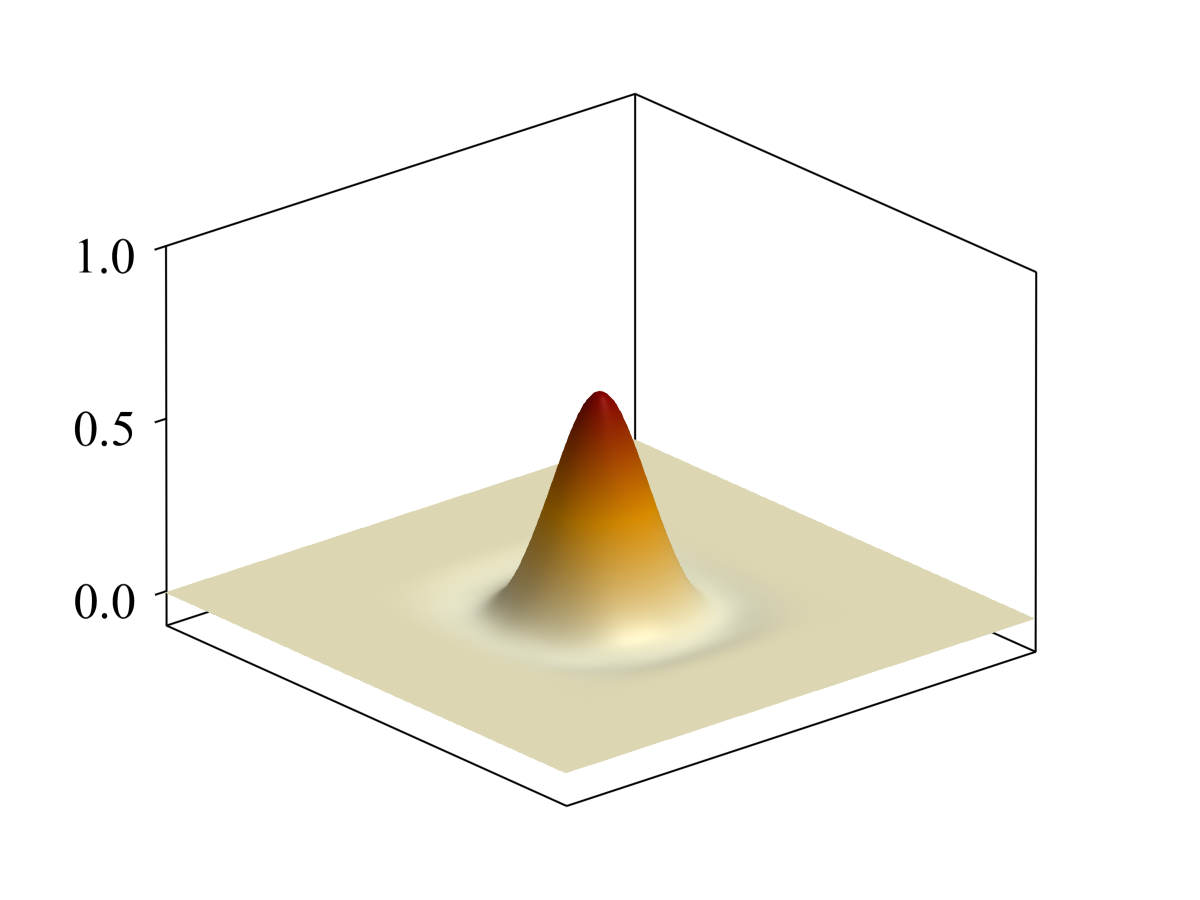
\includegraphics[scale=0.4]{figures/1.png}-大小、图片路径
\caption{\centering{边界点处无网格形函数}}-图名
\label{CHGraphsettings_fig1_meshfree}-命名
\end{figure}
\end{lstlisting}
\newpage
\subsection*{并排}
\begin{figure}[H]
    \centering
    \begin{subcaptiongroup}
    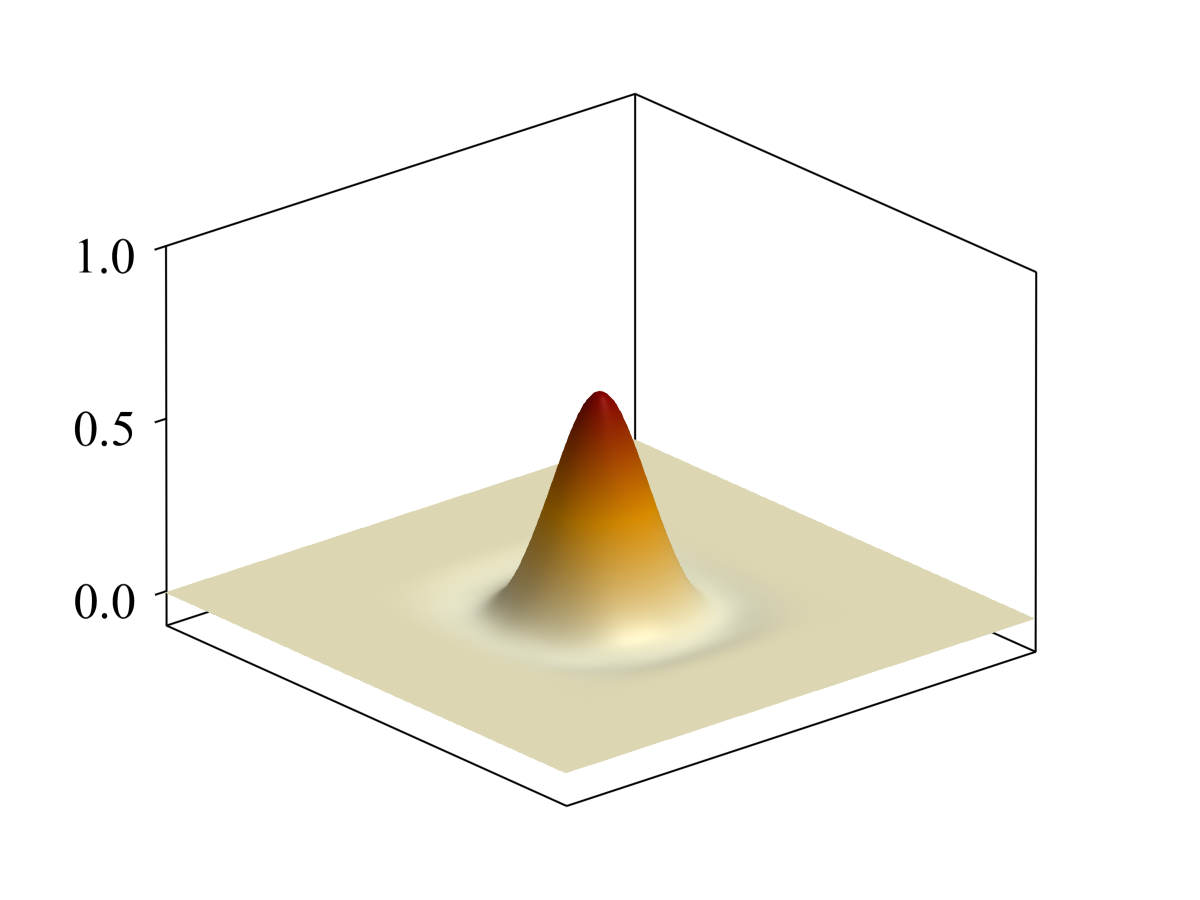
\includegraphics[width=0.49\textwidth]{figures/1.png}
    \phantomcaption\label{1}
    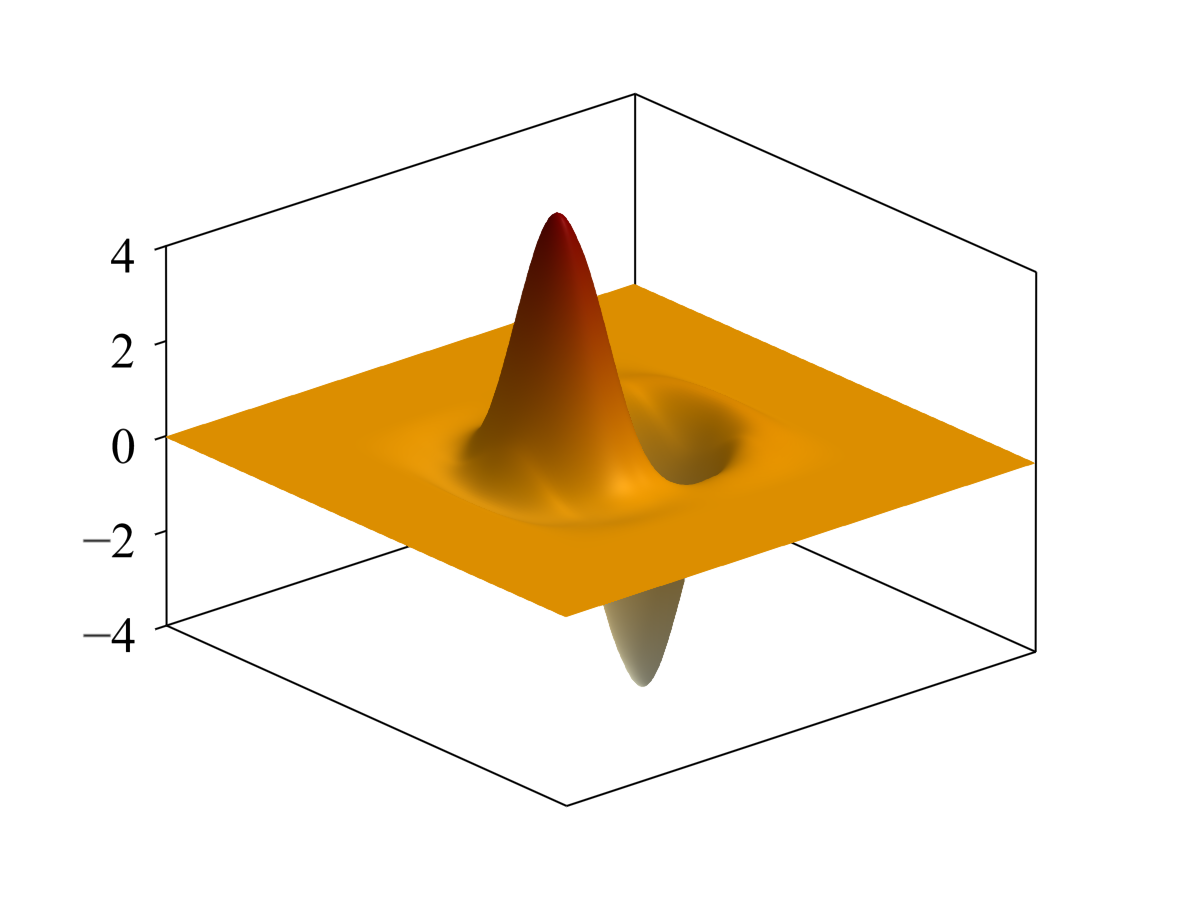
\includegraphics[width=0.49\textwidth]{figures/2.png}
    \phantomcaption\label{2}
    \end{subcaptiongroup}
\caption{\centering{无网格形函数:\subref{1}边界点;\subref{2}中心点}}
% NOTE:遇到图名过长需要换行的编写:
% \caption{\centering{标题:\protect\linebreak \subref{xxx} 小标题1;\subref{xx} 小标题2;\subref{xxx}小标题3;\subref{xxx} 小标题4}}
\label{CHGraphsettings_fig2_meshfree}
\end{figure}
并排图片Latex代码
\begin{lstlisting}
\begin{figure}[H]
\centering
\begin{subcaptiongroup}
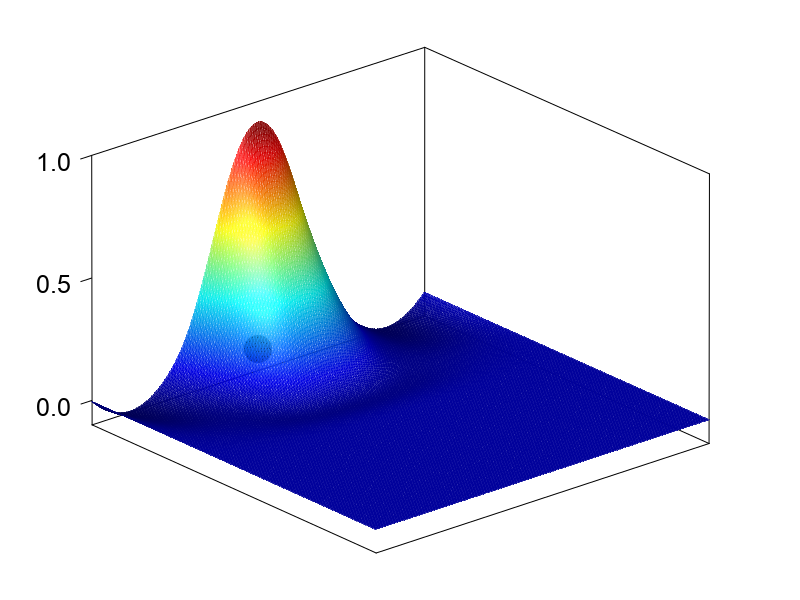
\includegraphics[width=0.49\textwidth]{figure/1.png}
\phantomcaption\label{1}
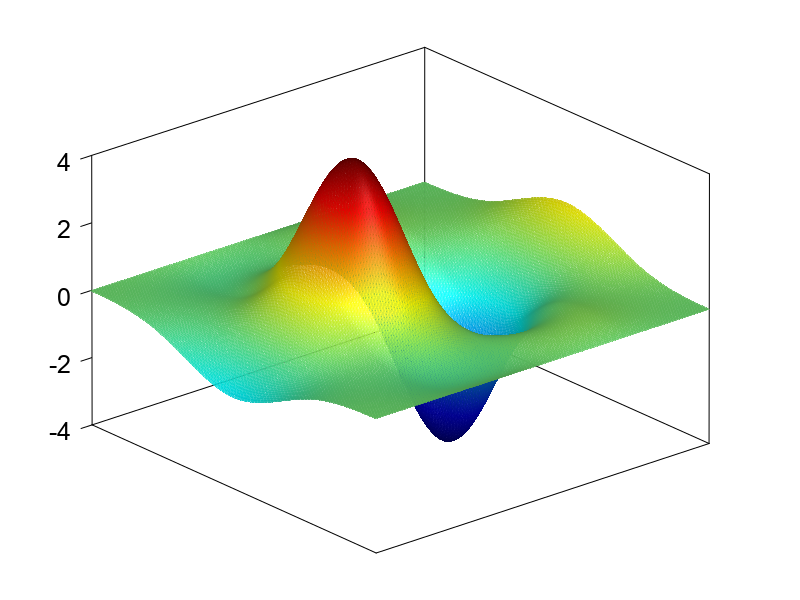
\includegraphics[width=0.49\textwidth]{figure/2.png}
\phantomcaption\label{2}
\end{subcaptiongroup}
\caption{\centering{无网格形函数:\subref{1}边界点;\subref{2}中心点}}
\end{lstlisting}
\newpage
\subsection*{表格式图片}
\begin{figure}[H]
    \centering
    \begin{tabular}{cccc}
    $\quad$&$p=2$&$p=2$&$p=2$\\
    边界点&\begin{subcaptiongroup}\raisebox{-0.5\height}{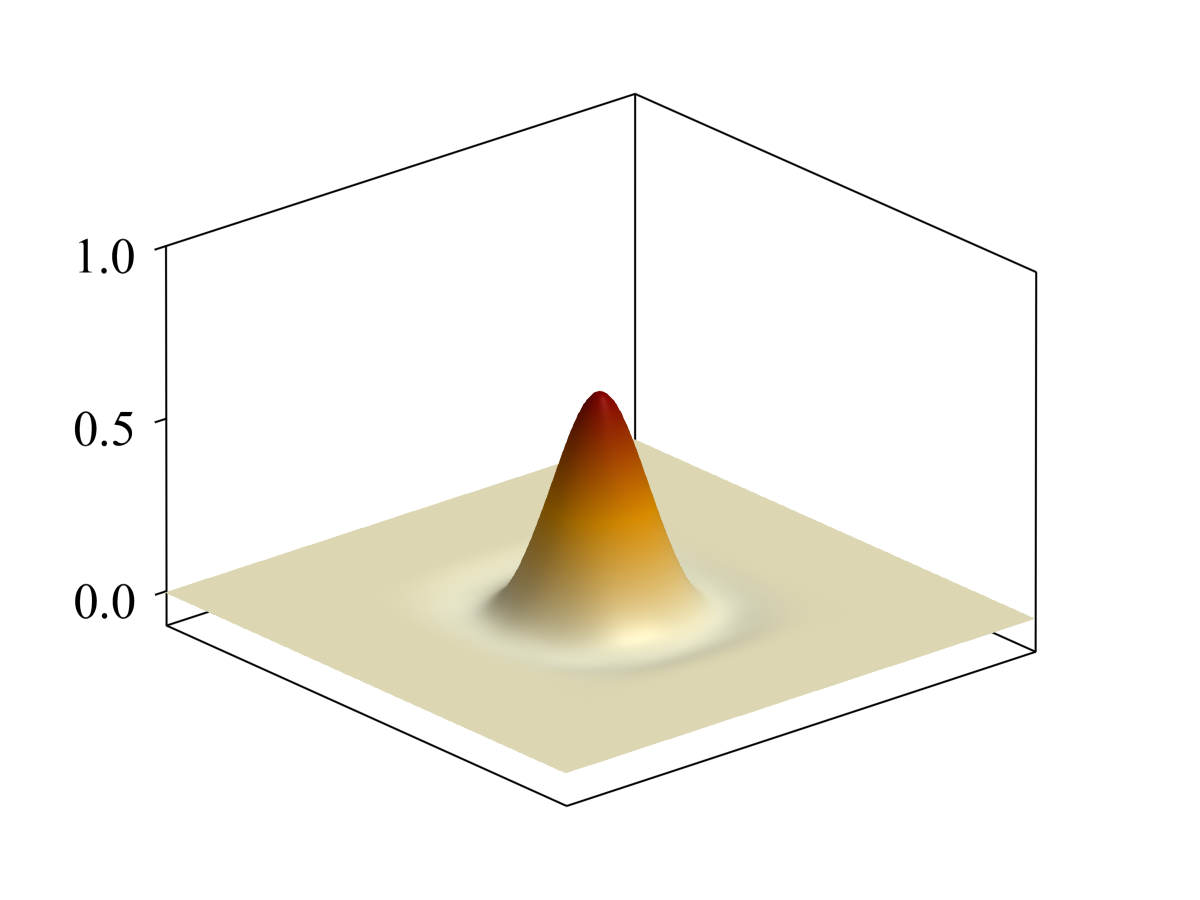
\includegraphics[width=0.3\textwidth]{figures/1.png}}\end{subcaptiongroup}
    &\begin{subcaptiongroup}\raisebox{-0.5\height}{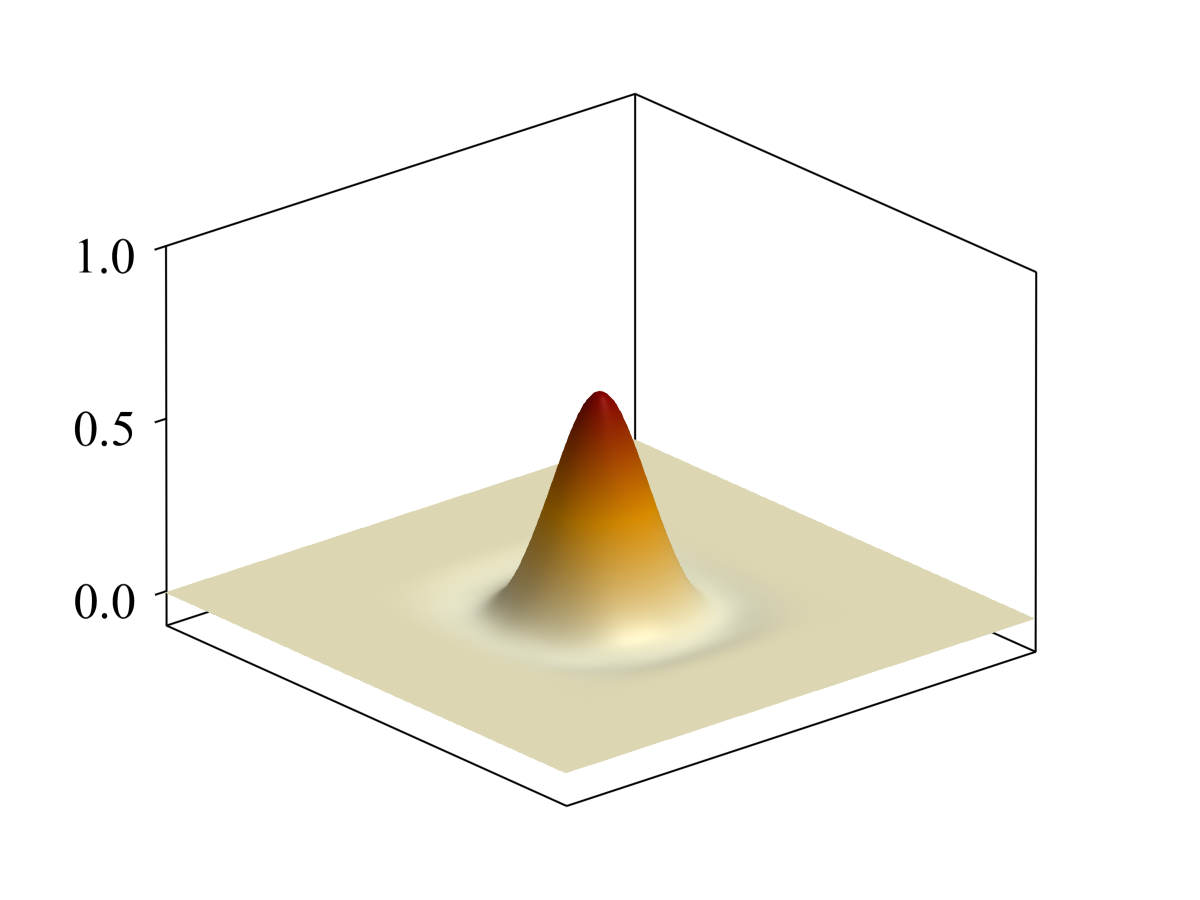
\includegraphics[width=0.3\textwidth]{figures/1.png}}\end{subcaptiongroup}
    &\begin{subcaptiongroup}\raisebox{-0.5\height}{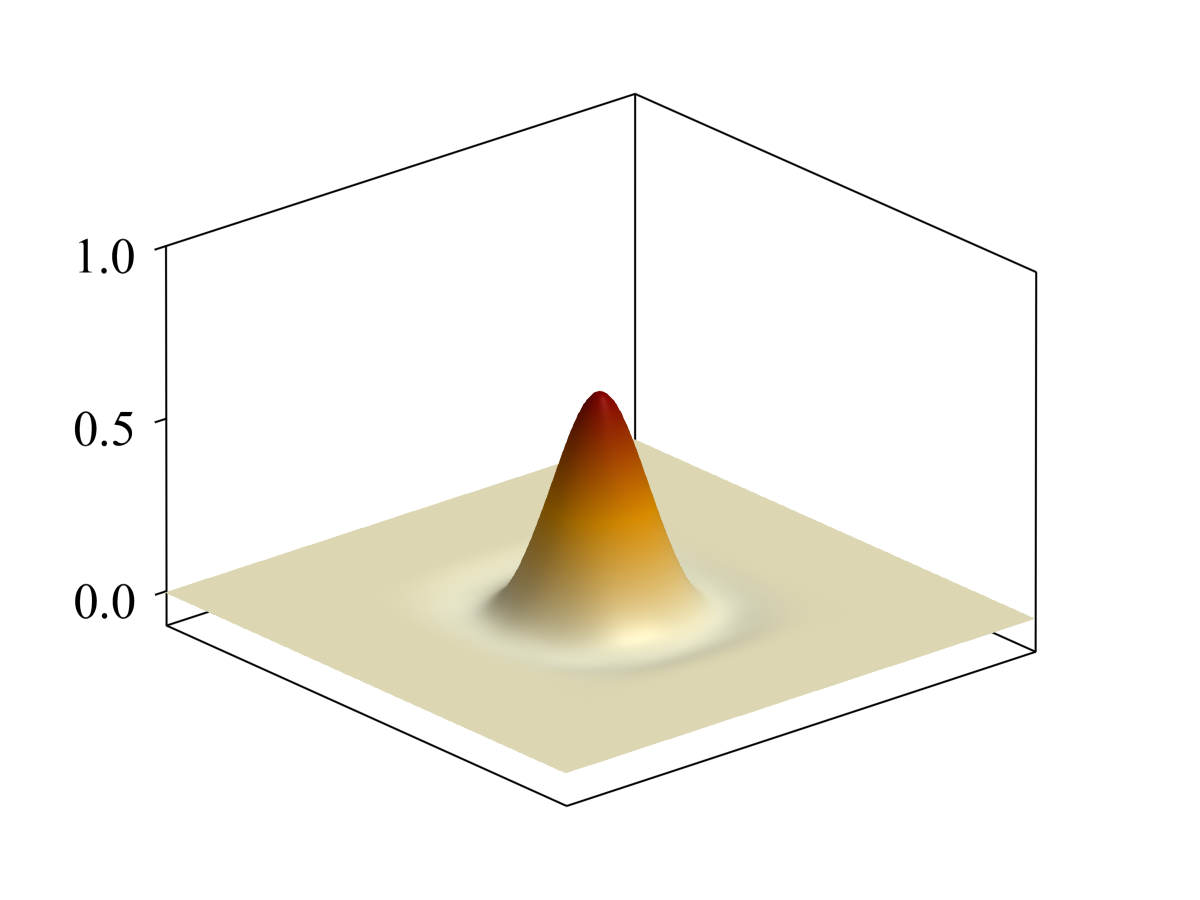
\includegraphics[width=0.3\textwidth]{figures/1.png}}\end{subcaptiongroup}\\
    中心点&\begin{subcaptiongroup}\raisebox{-0.5\height}{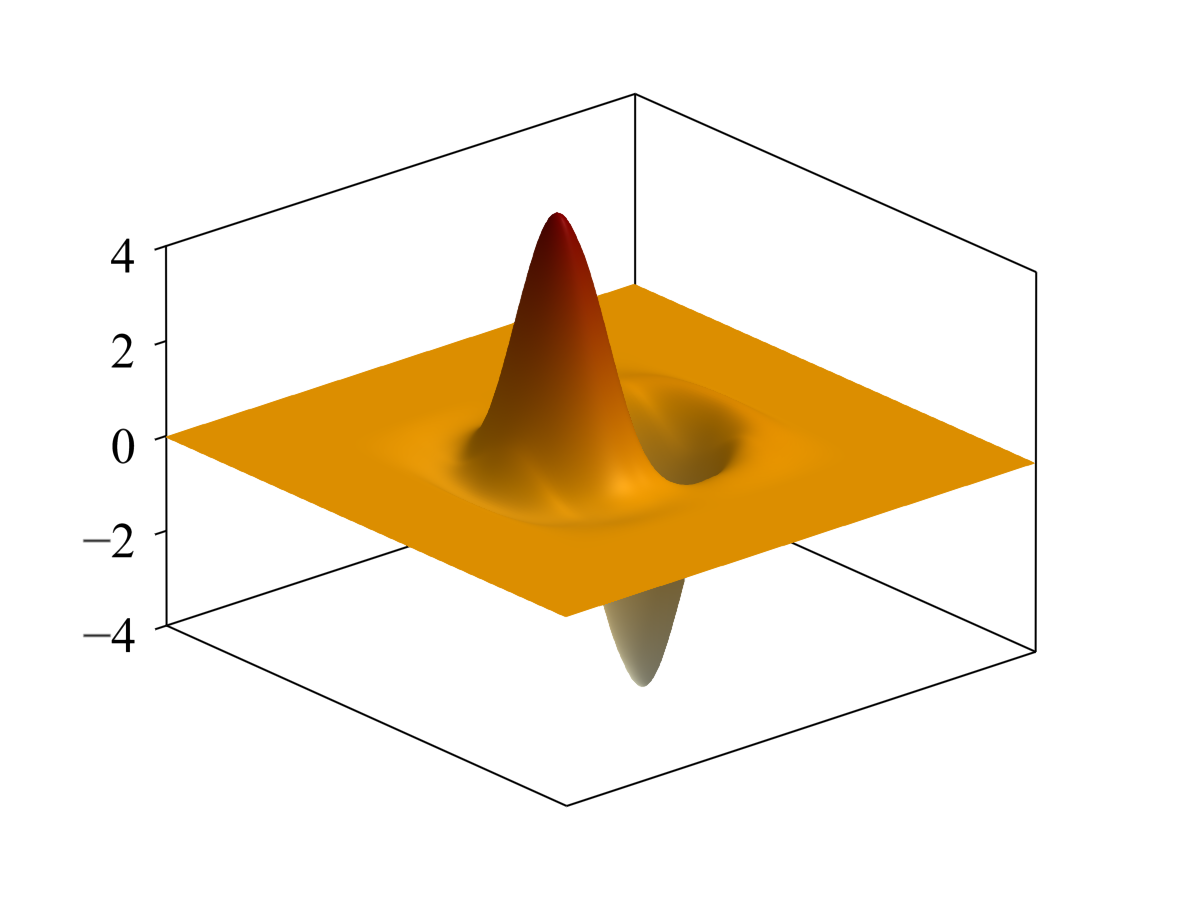
\includegraphics[width=0.3\textwidth]{figures/2.png}}\end{subcaptiongroup}
    &\begin{subcaptiongroup}\raisebox{-0.5\height}{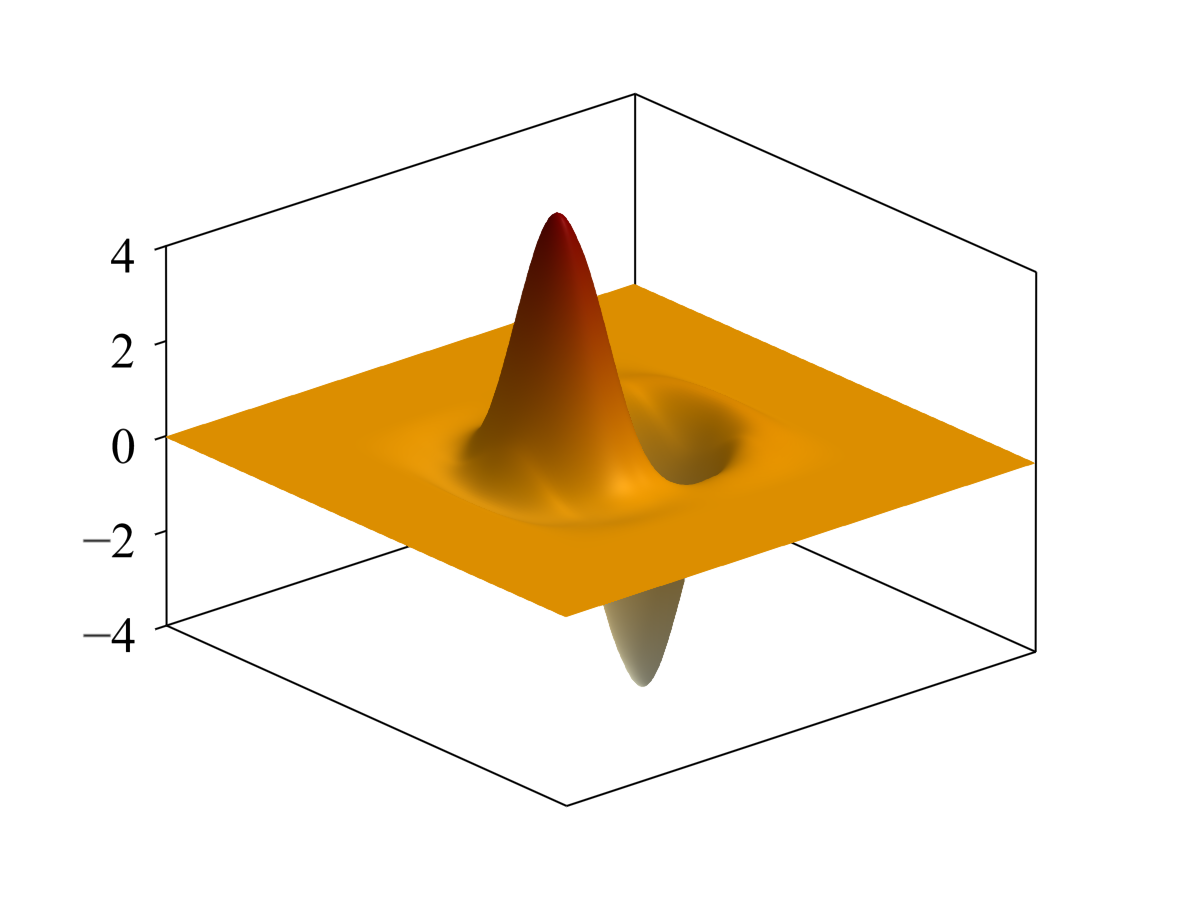
\includegraphics[width=0.3\textwidth]{figures/2.png}}\end{subcaptiongroup}
    &\begin{subcaptiongroup}\raisebox{-0.5\height}{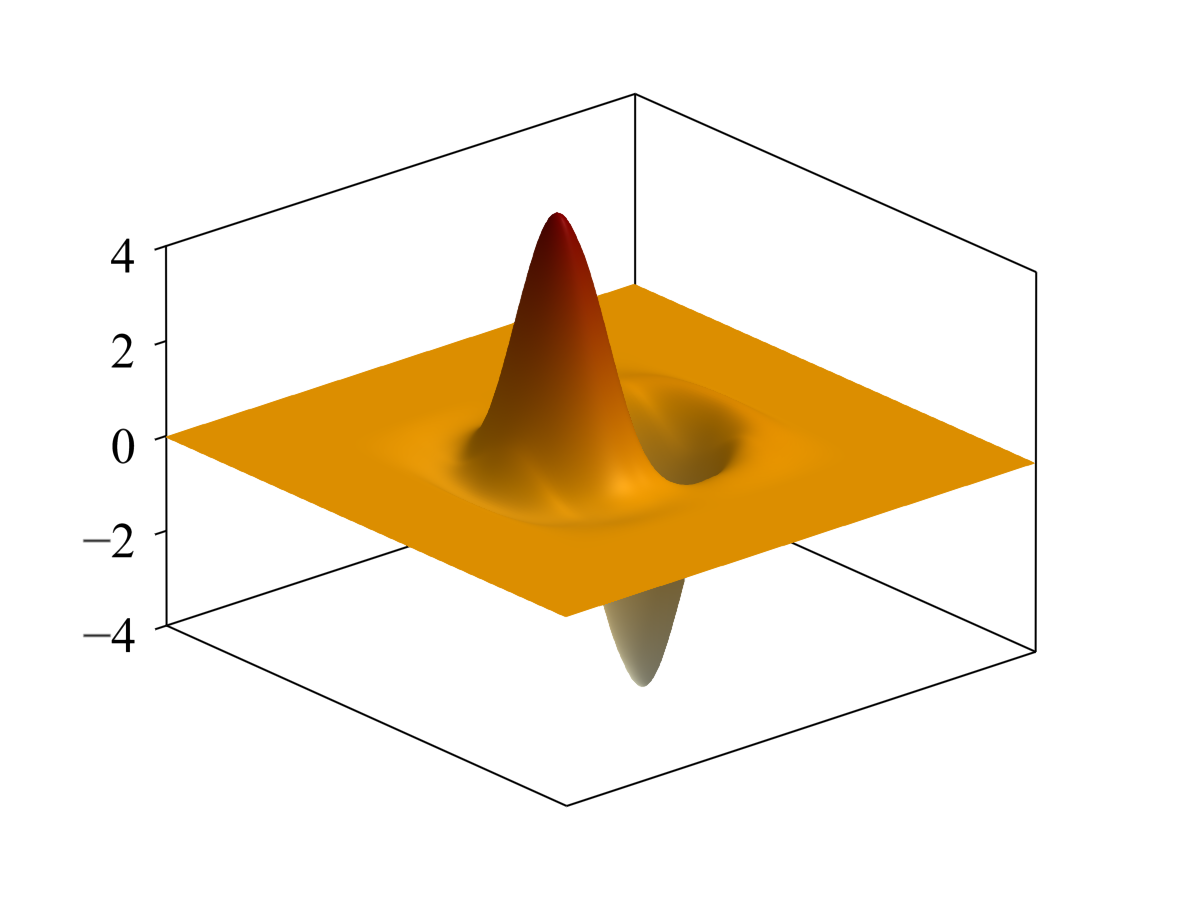
\includegraphics[width=0.3\textwidth]{figures/2.png}}\end{subcaptiongroup}\\
    \end{tabular}
    \caption{\textbf{二维边界点与内部节点无网格形函数图}}\label{CHGraphsettings_fig3_meshfree}
    \end{figure}

表格式图片Latex代码
\begin{lstlisting}
\begin{figure}[H]
\centering
\begin{tabular}{cccc}
$\quad$&$p=2$&$p=2$&$p=2$\\
边界点&\begin{subcaptiongroup}\raisebox{-0.5\height}{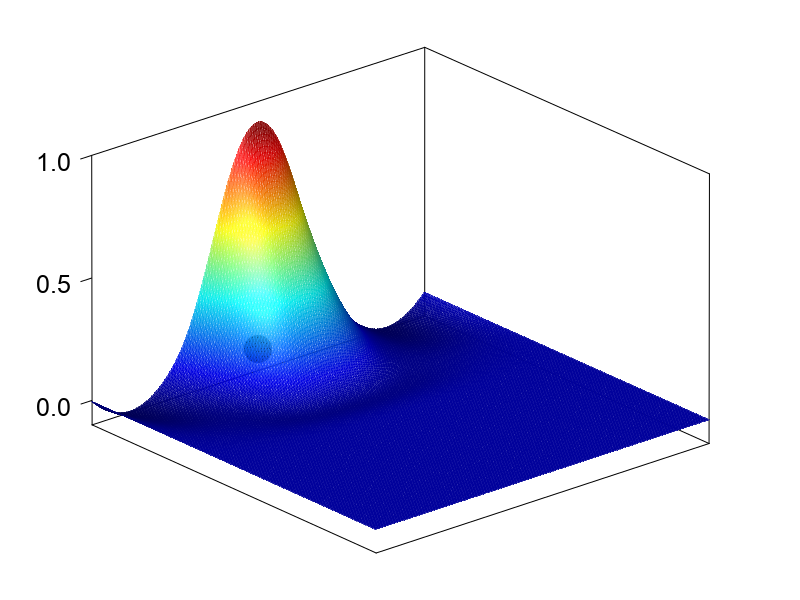
\includegraphics[width=0.3\textwidth]{figure/1.png}}\end{subcaptiongroup}
&\begin{subcaptiongroup}\raisebox{-0.5\height}{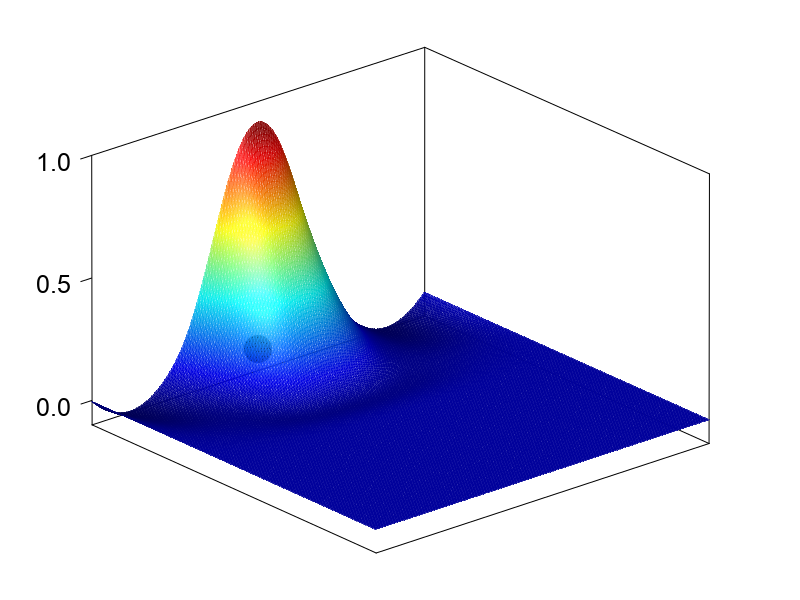
\includegraphics[width=0.3\textwidth]{figure/1.png}}\end{subcaptiongroup}
&\begin{subcaptiongroup}\raisebox{-0.5\height}{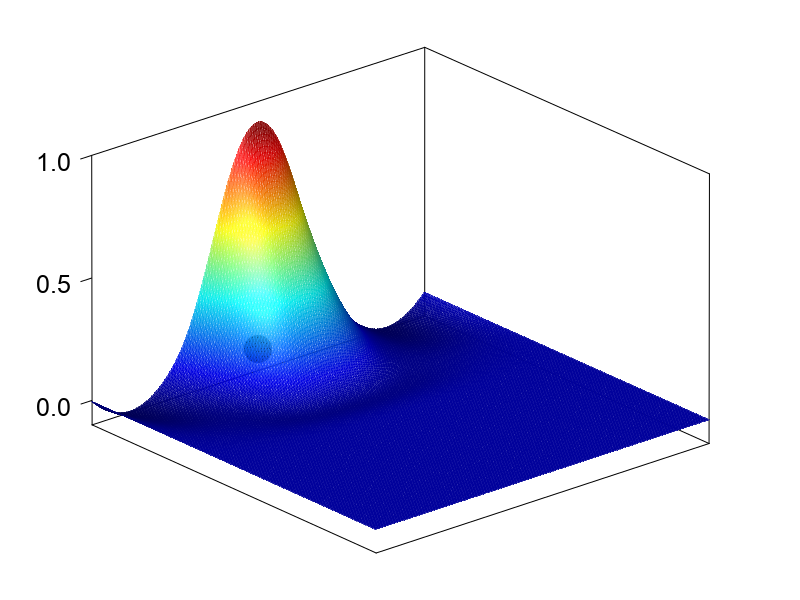
\includegraphics[width=0.3\textwidth]{figure/1.png}}\end{subcaptiongroup}\\
中心点&\begin{subcaptiongroup}\raisebox{-0.5\height}{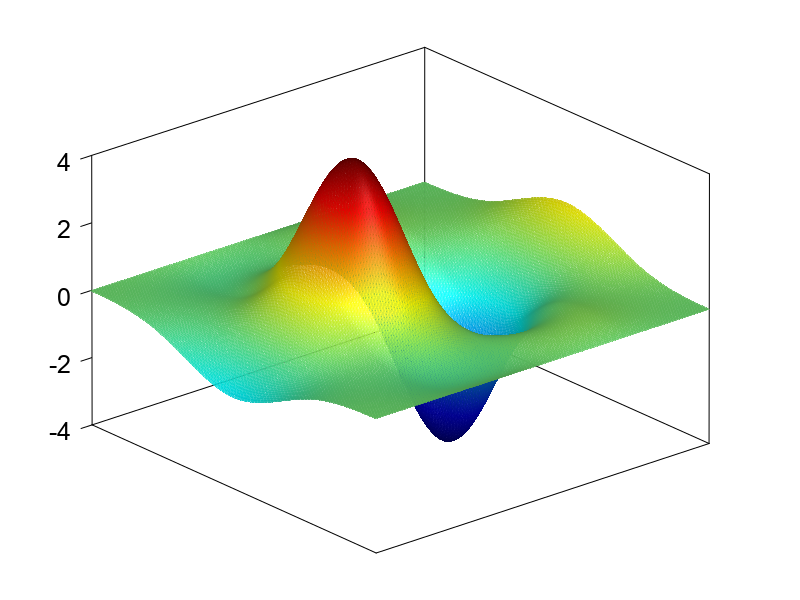
\includegraphics[width=0.3\textwidth]{figure/2.png}}\end{subcaptiongroup}
&\begin{subcaptiongroup}\raisebox{-0.5\height}{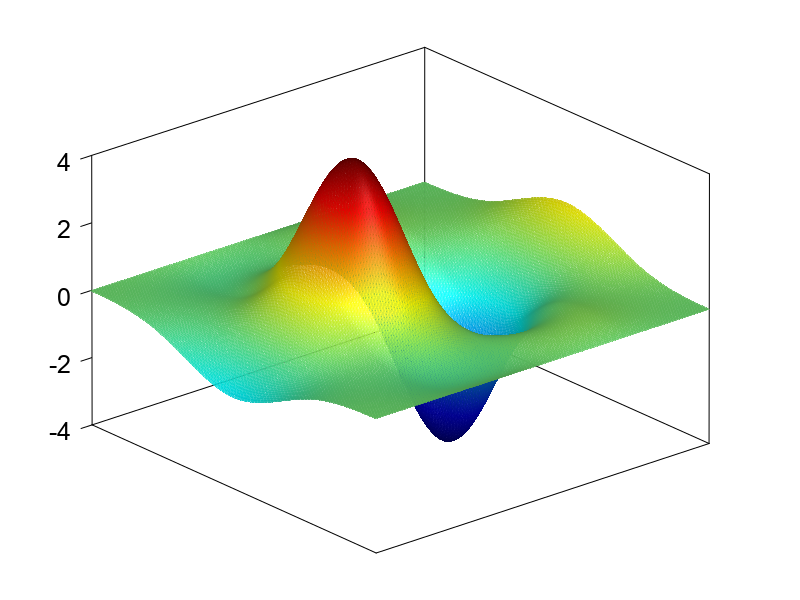
\includegraphics[width=0.3\textwidth]{figure/2.png}}\end{subcaptiongroup}
&\begin{subcaptiongroup}\raisebox{-0.5\height}{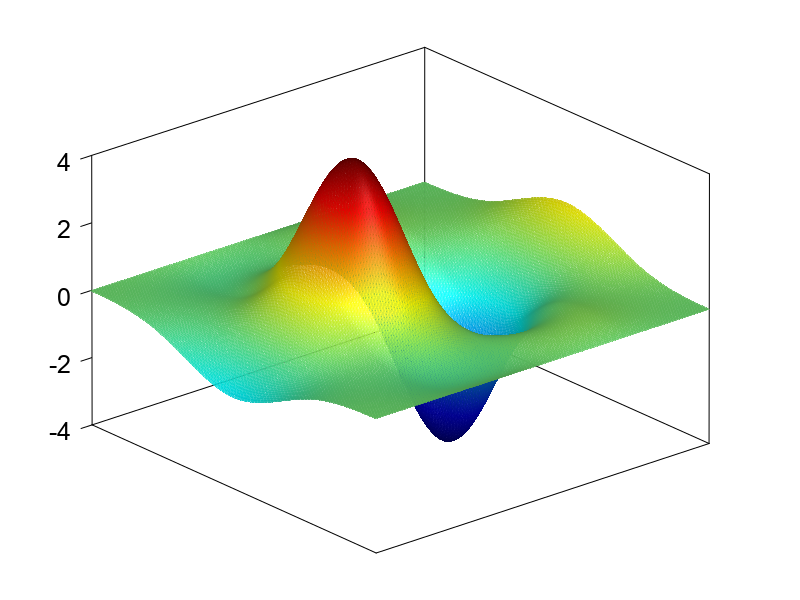
\includegraphics[width=0.3\textwidth]{figure/2.png}}\end{subcaptiongroup}\\
\end{tabular}
\caption{\textbf{二维边界点与内部节点无网格形函数图}}\label{CHGraphsettings_fig3_meshfree}
\end{figure}     
\end{lstlisting}

\subsection*{三线表}
\begin{table}[H]
    \caption{\textbf{三次基函数无网格法分片实验结果}}
    \centering\label{CHGraphsettings_table_cubic}
    \begin{tabular}{lcccc}
       \toprule
    & \multicolumn{2}{c}{二次分片实验} & \multicolumn{2}{c}{三次分片实验} \\ \cline{2-5}
       &$L_2$-Error$\quad$&$H_1$-Error&$L_2$-Error$\quad$&$H_1$-Error\\
       \midrule
      RKGSI-Penalty&$1.4\times10^{-7}$&$2.1\times10^{-6}$&$2.0\times10^{-7}$&$2.7\times10^{-6}$\\
      RKGSI-LM&$3.0\times10^{-4}$&$9.8\times10^{-3}$&$4.2\times10^{-4}$&$9.8\times10^{-3}$\\
      RKGSI-Nitsche&$3.6\times10^{-15}$&$1.0\times10^{-13}$&$4.6\times10^{-15}$&$9.5\times10^{-14}$\\
      RKGSI-HR&$3.1\times10^{-15}$&$1.0\times10^{-13}$&$3.5\times10^{-15}$&$7.4\times10^{-14}$\\
       \bottomrule
    \end{tabular}
    \end{table}
三线表Latex代码
\begin{lstlisting}
\begin{table}[H]
\caption{\textbf{三次基函数无网格法分片实验结果}}
\centering\label{CHGraphsettings_table_cubic}
\begin{tabular}{lcccc}
\toprule
& \multicolumn{2}{c}{二次分片实验} & \multicolumn{2}{c}{三次分片实验} \\ \cline{2-5}
&$L_2$-Error$\quad$&$H_1$-Error&$L_2$-Error$\quad$&$H_1$-Error\\
\midrule
RKGSI-Penalty&$1.4\times10^{-7}$&$2.1\times10^{-6}$&$2.0\times10^{-7}$&$2.7\times10^{-6}$\\
RKGSI-LM&$3.0\times10^{-4}$&$9.8\times10^{-3}$&$4.2\times10^{-4}$&$9.8\times10^{-3}$\\
RKGSI-Nitsche&$3.6\times10^{-15}$&$1.0\times10^{-13}$&$4.6\times10^{-15}$&$9.5\times10^{-14}$\\
RKGSI-HR&$3.1\times10^{-15}$&$1.0\times10^{-13}$&$3.5\times10^{-15}$&$7.4\times10^{-14}$\\
\bottomrule
\end{tabular}
\end{table}    
\end{lstlisting}

\chapter{使用Zotero管理参考文献}
1.下载附件:Better BibTex
链接:\href{https://zhuanlan.zhihu.com/p/621145900}{Better BibTex安装步骤}

2.新建分类建立文件库:references

3.右击该文件库-选择导出分类-以Better BibTex形式导出条目

4.导出条目至与Latex文件相同路径

5.在主文件(ef:main.tex)中添加:
\begin{lstlisting}
\begin{document}
    .....
    \bibliography{references}--导出文献的文件名
    .....
\end{document}
\end{lstlisting}
eg:基于赫林格-赖斯纳原理的变分一致型伽辽金无网格法\cite{Wu2022,wu2023}相较于传统的本质边界条件施加方法能够有效提高计算精度和计算效率。

Latex代码

\begin{lstlisting}
eg:基于赫林格-赖斯纳原理的变分一致型伽辽金无网格法\cite{Wu2022,wu2023}相较于传统的本质边界条件施加方法能够有效提高计算精度和计算效率。
\end{lstlisting}

\chapter{\LaTeX 部分所需包介绍}


编写公式-\{amsmath,amsfonts,amssymb,textcomp,ulem\}

绘制表格-\{booktabs,multirow,tabularx,float\}

书写代码-\{listings\}

代码块设置
\begin{lstlisting}
\lstset{breaklines,        %自动换行
        columns=flexible,  %不随便添加空格,只在已经有空格的地方添加空格,
       }
\end{lstlisting}

设置PDF文档中超链接的颜色
\begin{lstlisting}
\hypersetup{colorlinks=true,linkcolor=black,citecolor=black}
\end{lstlisting}



% NOTE 毕业论文致谢部分
% \begin{acknowledgements}
感谢
\end{acknowledgements}

\appendix
\chapter{附录}
附录章节前需添加以下下代码
\begin{lstlisting}
    \appendix
\end{lstlisting}


\chapter{参考格式}
\begin{lstlisting}

\documentclass[engineeringmaster]{hquThesis}-hquThesis是模板文件,包含文本格式,字体设置,文献格式.....
\usepackage{amsmath,amsfonts,amssymb,textcomp}-公式所需
\usepackage{booktabs,multirow,tabularx,float}-表格所需
\hypersetup{colorlinks=true,linkcolor=black,citecolor=black}-设置超链接格式
\titleZh{XXX}-中文标题
\titleEn{XXX}-英文标题
\id{}-学号
\authorZh{XXX}-作者姓名
\supervisorZh{XXX}{XXX}-指导教师+职称
\cosupervisorZh{XXX}{XXX}-合作教师+职称
\practicevisorZh{XXX}{XXX}-实践教师+职称
\departmentZh{土木工程学院}
\fieldZh{结构体系创新与工程应用}
\majortype{工程硕士}
\major{土木水利}
\coverdate{二〇二四年三月XX日}
-封面设置
\begin{document}-正文开始

\makecover
{
    \begin{center}
        \sffamily\fontsize{16pt}{25pt}\selectfont 学\hspace{8pt}位\hspace{8pt}论\hspace{8pt}文\hspace{8pt}答\hspace{8pt}辩\hspace{8pt}委\hspace{8pt}员\hspace{8pt}会\hspace{8pt}决\hspace{8pt}议
    \end{center}
} \vspace{32pt}
{
    \fontsize{14pt}{26pt}\selectfont
    \noindent\hspace{28pt}\rmfamily 根据《中华人民共和国学位条例》、《中华人民共和国学位条例暂行实 施办法》、《华侨大学学位授予工作细则》及《华侨大学研究生学位论文质 量监控与评阅答辩的管理规定》的规定,学位论文答辩委员会经充分交换意 见,对论文做出评价,并以无记名投票方式进行表决,同意该同学通过\degree 学位论文答辩,同意授予\degree 学位。\par
    \vspace{192pt}
    \noindent\flushright 答辩委员会(主席签字):\underline{\hspace{156pt}}\vspace{14pt} \par
    \noindent\flushright 答辩时间:\underline{\hspace{60pt}}年\underline{\hspace{25pt}}月\underline{\hspace{25pt}}日 \par
}
-答辩委员会
\noindent\fbox{%
    \parbox{14.3cm}{
    \vspace{24pt}\begin{center}\sffamily\fontsize{16pt}{\baselineskip}\selectfont 学位论文独创性声明\end{center}\vspace{18pt}
    \hspace{28pt}\declarationfont\fontsize{14pt}{28pt}\selectfont
    本人声明兹呈交的学位论文是本人在导师指导下完成的研究成果。论文写作中不包含其他人已经发表或撰写过的研究内容,如参考他人或集体的科研成果,均在论文中以明确的方式说明。本人依法享有和承担由此论文所产生的权利和责任。\par
    \vspace{28pt}\hspace{28pt} 论文作者签名:\underline{\hspace{112pt}}\hspace{7pt}签名日期:\underline{\hspace{77pt}}\par\vspace{7pt}
    }%
}
\par
\vspace{44pt}
\noindent\framebox[\linewidth]{
    \parbox{14.3cm}{
    \vspace{24pt}\begin{center}\sffamily\fontsize{16pt}{\baselineskip}\selectfont 学位论文版权使用授权声明\par\end{center}\vspace{18pt}
    \hspace{28pt}\declarationfont\fontsize{14pt}{28pt}\selectfont 
    本人同意授权华侨大学有权保留并向国家机关或机构送交学位论文的复印件和电子版,允许学位论文被查阅和借阅。本人授权华侨大学可以将本学位论文的全部内容或部分内容编入有关数据库进行检索,可以采用影印、缩印或扫描等复制手段保存和汇编本学位论文。\par\vspace{28pt}
    \hspace{28pt}论文作者签名:\underline{\hspace{84pt}}\hspace{7pt}指导老师签名:\underline{\hspace{84pt}}\par
    \hspace{28pt}签\hspace{7pt}名\hspace{7pt}日\hspace{7pt}期:\underline{\hspace{91pt}}\hspace{7pt}签\hspace{7pt}名\hspace{7pt}日\hspace{7pt}期:\underline{\hspace{91pt}}\par\vspace{7pt}
    }
}
-独创性说明
\frontmatter

\begin{abstract}
自锁问题是有限元分析中的一类常见数值问题,主要表现为在模拟某些特定物理现象时,数值解因过度约束而丧失精度或收敛性。
常见的自锁问题包括以下两类:体积自锁:在模拟不可压缩材料时,由于体积应变能的过度约束,导致数值解出现刚化现象,无法准确描述材料的变形特性;剪切自锁:在模拟中厚板结构时,由于剪切应变能的过度约束,导致数值解无法准确反映结构的实际变形行为。
混合有限元法是解决自锁问题的常用方法,通过引入额外的场变量(如压力场)来减少过度约束。
例如,在不可压问题中,使用位移--压力混合离散可以有效缓解体积自锁现象。
然而,混合有限元法必须满足LBB稳定性条件,才能保证数值解的稳定性,在一定情况下也可能会产生压力振荡现象。因此,选择合适的变量间约束比至关重要。
尽管混合有限元法常用于解决自锁问题,但并非所有混合离散方案都满足LBB稳定性条件,而已知的满足LBB稳定性条件的混合离散方案常常表现出过度约束的状态。
无网格法具有不依赖于几何拓扑关系的高阶光滑形函数,能够任意的布置节点,特别适用于变量间的混合离散过程。通过结合无网格法与混合有限元法,可以有效解决传统方法中的问题。

本文针对传统混合离散方案存在的问题,提出了一种有限元无网格混合离散分析方法。
并在该方法的基础上,研究了体积不可压问题和中厚板剪切自锁问题中离散节点分布与LBB稳定性条件之间的关系,建立了考虑最优约束比的LBB稳定性条件验证方法,从而确定免自锁的最优约束比范围。
依托再生核无网格法理论框架,通过调整约束比,生成了一种免自锁且满足LBB稳定性条件的有限元无网格混合离散方案。
最后,通过体积不可压问题和中厚板问题的系列经典算例,验证了所提LBB稳定性条件验证方法的正确性,以及有限元无网格混合离散方案的计算精度和稳定性。

\end{abstract}
\keywords{自锁问题;混合离散;最优约束比;LBB稳定性条件;无网格法}

\begin{abstractEn}
Locking problems are a common class of numerical issues in finite element analysis, primarily manifested as a loss of accuracy or convergence in numerical solutions due to excessive constraints when simulating specific physical phenomena. 
Typical locking problems include two categories: volumetric locking, where numerical solutions exhibit artificial stiffening due to over-constrained volumetric strain energy in modeling incompressible materials, and shear locking, where numerical solutions fail to accurately reflect the deformation behavior of moderately thick plate structures due to over-constrained shear strain energy. 
The mixed finite element method is widely used to address locking problems by introducing additional field variables (e.g., pressure fields) to relax excessive constraints. For instance, displacement-pressure mixed discretization effectively mitigates volumetric locking in incompressible problems. 
However, the mixed finite element method must satisfy the LBB (Ladyzhenskaya-Babuška-Brezzi) stability conditions to ensure numerical stability, and pressure oscillations may still occur under certain circumstances. 
Therefore, selecting an appropriate constraint ratio between variables is critical. Although the mixed finite element method is commonly employed to resolve locking problems, not all mixed discretization schemes satisfy the LBB stability conditions. Even known LBB-compliant schemes often exhibit over-constrained states.
Meshfree methods, characterized by high-order smooth shape functions independent of geometric topology and flexible node arrangement, are particularly suitable for mixed discretization processes involving multiple variables. By integrating meshfree methods with the mixed finite element approach, traditional limitations can be effectively addressed.

This study proposes a finite element-meshfree hybrid discretization method to tackle the shortcomings of conventional mixed discretization schemes. 
Building on this method, the relationship between discrete node distributions and LBB stability conditions is systematically investigated for both incompressible problems and moderately thick plate shear locking problems.
A verification framework for LBB stability conditions incorporating an optimal constraint ratio is established to determine the optimal constraint range for locking-free solutions. 
Leveraging the theoretical framework of the reproducing kernel meshfree method, a locking-free hybrid discretization scheme satisfying LBB stability conditions is developed by adjusting the constraint ratio. 
Finally, a series of benchmark cases for incompressible problems and moderately thick plate problems validate the correctness of the proposed LBB stability verification framework and demonstrate the computational accuracy and stability of the finite element-meshfree hybrid discretization scheme.

\end{abstractEn}
\keywordsEn{Locking problems; Mixed discretization;  Optimal constraint ratio;LBB stability conditions; Meshfree method}
-摘要
\tableofcontents
\mainmatter
\chapter{引言}
\section{选题背景及意义}
自锁现象是有限元分析中常见的一种数值问题,通常表现为在模拟某些特定材料行为或几何特性时,计算结果过于刚硬,导致变形被不合理地抑制,从而无法准确反映实际物理行为。本文考虑两类常见的自锁问题:体积自锁问题和剪切自锁问题。

体积自锁问题主要发生在模拟体积不可压材料或近似不可压材料的过程中。
体积不可压材料是指在变形过程中体积膨胀收缩受约束的一类材料,如建筑结构中的隔振橡胶支座、用于提高电子元件与散热器之间热传导效率的导热硅脂,以及药物控释系统中的高分子水凝胶等,均可视为是体积不可压材料。这类材料在土木工程、电子工程、生物医疗等领域有着广泛的应用。
通过对不可压材料的结构进行深入分析,可以有效缩短试制周期,减少材料消耗,降低实验成本,提高开发效率。
然而,在实际分析过程中,由于复杂几何结构、非线性应力应变关系等一系列问题的存在,往往难以获得解析解。
因此,数值仿真分析成为了研究体积不可压材料的重要工具。在数值分析中,体积约束施加不当常导致计算结果精度下降,这一问题被称为体积不可压问题或不可压问题。
为了满足工业生产及科学研究中对不可压材料的应用需求,发展不可压问题高精度、高效率的数值分析方法,成为了计算力学领域的重要研究课题。

剪切自锁问题主要发生在模拟中厚板受弯的过程中。
中厚板是建筑结构中主要的基本构件,这类构件主要承受竖向荷载,变形以受弯为主。
在传统的Kirchhoff假设下,板构件忽略由横向剪切应力引起的剪切变形。
然而,当板构件的宽厚比在0.05-0.2时,受弯作用下梁内轴向剪切力所产生的变形将引起附加挠度,使变形后的平截面不与轴线垂直,不符合平截面假定。
此时,Kirchhoff假设已经不再适用,需要采用考虑剪切变形的Mindlin假设。
同样,数值仿真方法是一种简单、快速、低成本的结构受力分析方法,是结构设计中重要的理论依据,而有限元法\cite{hughes2000}是目前最成熟、应用最广泛的数值仿真分析方法。
在Mindlin假设下,传统有限元法中具有位移和转角两类自由度,能捕捉由结构的剪切变形,适用性高于Kirchhoff假设。
然而,由于位移自由度与转角自由度所对应刚度的量纲并不相同,当处理薄板时,不同自由度所对应量纲的量级差将变大,从而导致大量纲项所对应的自由度受到约束。
过多的自由度被约束时,将引起有限元分析出现严重的剪切自锁现象\cite{arnold1997}。剪切自锁问题将引起有限元分析精度严重下降,严重阻碍有限元法在中厚板问题中的发展。

当前,缓解自锁现象的主流方法是混合离散方法。对于体积不可压问题,通常采用位移--压力混合离散框架;而对于中厚板问题,则采用挠度--剪切应力混合离散框架。为确保数值求解的计算精度和稳定性,混合离散框架需要满足Ladyzhenskaya--Babuska--Brezzi(LBB)稳定性条件。
以体积不可压问题为例,体积膨胀收缩过程会约束压力自由度,而压力自由度与位移自由度的数量比称为体积约束比(或约束比)。当体积约束比过高时,无法满足LBB稳定性条件,从而出现体积自锁现象\cite{hughes2000,bathe1996}。反之,当约束比过低时,则会引起沙漏模态,导致计算结果的不稳定\cite{Pantuso1997}。
Hughes\cite{hughes2000}通过对不可压问题的连续微分方程进行分析,提出在二维情况下,当约束比趋近于2时,可以避免体积自锁现象,并得到稳定的计算结果。
然而,这一结论仅适用于无限自由度的连续情况,对于数值模拟中有限自由度情况并不完全适用。
例如,当位移与压力采用相同数量的离散节点\cite{bathe1996},或压力采用全域连续的形函数进行离散时\cite{Huerta2001,Taylor2011},尽管体积约束比始终保持为2,但仍然出现体积自锁现象。
目前,以约束比大小作为标准来判断数值分析方法能否有效解决自锁问题的研究仍处于较为粗浅的阶段。
虽然在伽辽金弱形式中增加稳定性\cite{wu2013,Rossi2021},或采用特殊基函数的形函数进行离散\cite{Vidal2002}可以规避LBB稳定性条件,但这会导致弱形式与求解空间的改变,并可能引入额外的误差。
因此,研究混合离散方法中约束比与LBB稳定性条件之间的关系,以确定最优约束比,是发展免自锁问题数值分析方法的迫切需求。

\begin{figure}[!h]
    \centering 
        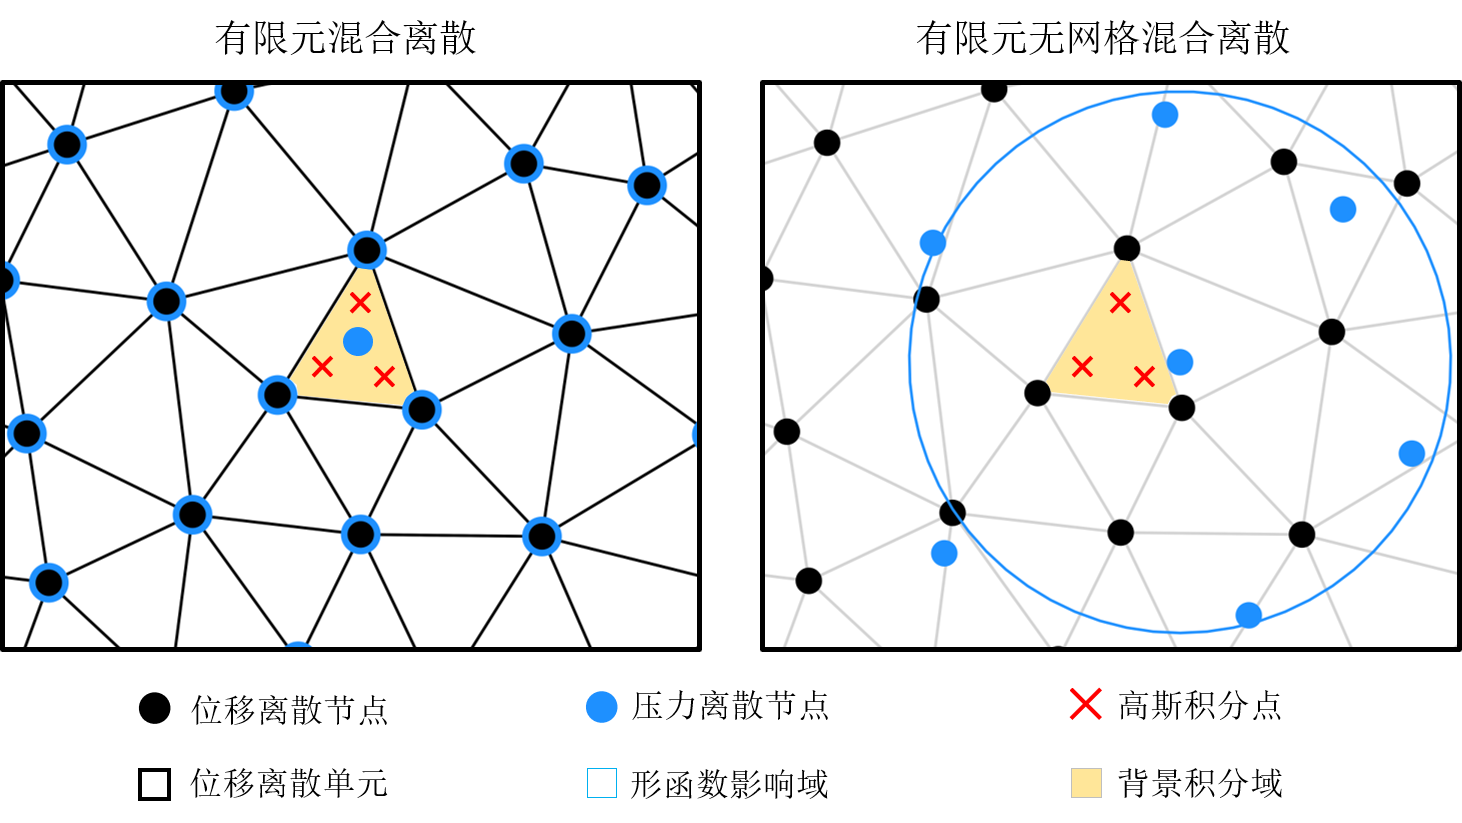
\includegraphics[scale=0.6]{figures/mix_ex.png}
        \caption{混合离散示意图}\label{ch_1:fig:mix}
\end{figure}
混合离散方法中的数值离散方法为有限元法,该方法采用单元的拓扑信息构建形函数,具有形式简洁、计算高效的特点。
然而,有限元形函数依赖于单元插值,这一特点使其在免自锁问题的应用中存在诸多局限性。
如图\ref{ch_1:fig:mix}所示,在体积不可压问题的位移--压力有限元混合离散框架下,压力节点离散过程依赖于位移节点。
为了简化高斯积分点处的形函数计算过程,位移、压力离散单元及背景积分域的轮廓需要重合,这将导致约束比无法被灵活调整,从而限制了其在实际问题中的应用。
相比之下,无网格法\cite{Belytschko1994,liu1995,zhang2004,chen2017}通过节点信息构建高阶连续光滑的形函数,不仅简化复杂区域的离散过程和局部细化过程,还能有效缓解网格畸变引起的精度下降问题,适用于复杂结构大变形分析,近年来得到了快速地发展\cite{liu2011,chen2014,yu2017,yang2016,wang2017,gao2019,wang2019,deng2019,chen2021,cao2020,li2020}。
如图\ref{ch_1:fig:mix}所示无网格有限元混合离散过程,压力节点离散无需依赖位移节点和背景积分域,即位移和压力形函数的影响域与背景积分域高度不重合,高斯积分点处位移和压力形函数依旧直接通过积分点与节点的间距进行计算,算法实现过程简单且高效。
无网格法凭借其基于节点构建形函数的特点,提高了混合离散的便利性,适用于调整优化混合离散过程的约束比。

本文研究免自锁问题的混合离散最优约束比与可任意调整优化约束比,建立一种自稳定有限元无网格混合离散分析方法,为自锁问题提供一种精确、鲁棒和高效的数值工具。
\section{国内外研究历史及现状}
为了缓解自锁问题,近年来国内外许多学者进行了广泛的研究,通常通过将约束比调整到适当的水平。
在传统有限元法中,这种调整是基于单元进行的,而传统有限元法往往表现出过度约束的状态。
调整约束比的方法主要包括减少压力(或剪切应力)自由度或增加位移(或挠度)自由度两种途径。
降低混合公式中压力的近似节点数量可以有效缓解自锁现象,例如广泛使用的Q4P1单元(4节点四边形位移--1节点分段常数压力单元)和Q8P3单元。
此外,通过使用连续形函数连接每个单元中的局部压力节点,也可以减少压力自由度的总数并增加约束比,例如T6P3单元(6节点三角形位移--3节点连续线性压力单元)和Q9P4(TaylorHood单元)\cite{hood1974}。
这些方案属于混合离散框架,也可以通过投影的方式实现,其中压力近似值被投影至低阶空间中。例如选择积分法\cite{malkus1978,shilt2020}、B--bar或F--bar假定应变法\cite{simo1990,broccardo2009,coombs2018,saloustros2021,rodriguez2023}、压力投影法\cite{simo1985,dohrmann2004}和增强应变法\cite{lovadina2003}。
同样,以规则交叉布置的常规3节点三角形单元也可以减少压力自由度的数量\cite{bathe2001}。
需要注意的是,尽管上述方法缓解了自锁现象并获得了相对准确的位移解,但并非所有的方法都能满足LBB稳定性条件。例如,Q4P1单元的压力解就会出现明显的振荡现象,称为伪压力模式或棋盘模式\cite{bathe2001}。在这种情况下,需要额外的稳定方法来消除压力振荡。
例如,多尺度稳定化方法(VMS):Hughes\cite{hughes1995}提出了基于多尺度现象的变分方法,通过引入子网格尺度模型和稳定化方法,揭示了稳定化方法的理论起源,为处理物理和工程中的多尺度问题提供了新的理论基础;Masud和Xia\cite{masud2005}提出了多尺度/稳定有限元法,将位移场分解为粗和细尺度,并允许任意组合插值函数,使得不满足LBB稳定性条件的等阶插值变得稳定且收敛;Rossi等人\cite{Rossi2021}采用体积应变代替混合公式中的压力作为节点变量,并采用变分多尺度稳定化来解决体积不可压问题;Karabelas等人\cite{karabelas2022}提出使用稳定的P1--P1单元有限元框架缓解体积自锁现象。
此外,Hughes等人\cite{hughes1986}提出的伽辽金/最小二乘法(GLS),也可以用来消除压力振荡。

另一类有限元方法通过增加位移自由度来调整约束比。例如,基于3节点三角形单元,Arnold等人在每个单元中引入了三次气泡函数来增加位移自由度,被称为MINI单元\cite{arnold1984,auricchio2005}。研究表明,MINI单元属于VMS框架\cite{quarteroni1994},并且可以使用两级投影框架来解析证明其满足LBB稳定性条件。Crouzeix--Raviart 单元\cite{crouzeix1973}通过将节点从三角形顶点转移到边,增加了约束比,因为在三角形拓扑中,边的数量多于顶点的数量。

在过去的二十年里,国内外学者们提出了各种配备全局光滑形函数的新型近似方法,如移动最小二乘近似\cite{Belytschko1994}、再生核近似\cite{liu1995}、径向基函数\cite{chi2014,wang2020d}、最大熵近似\cite{ortiz-bernardin2015}和NURBS近似\cite{hughes2005,auricchio2010}等方法。
在这些方法中,由全局连续形函数导数估算的近似压力在二维不可压弹性问题中也保持了约束比为2。然而,相应的结果仍然显示了自锁引起的精度降低\cite{Huerta2001}。在这些方法中引入了广泛使用的有限元免自锁技术,以提高其性能。
例如,Moutsanidis等人采用选择积分方案和B--bar、F--bar方法来提高再生核粒子法\cite{moutsanidis2020,moutsanidis2021}。Wang等人将具有泡泡稳定函数的选择积分方案应用于基于节点的平滑粒子有限元法\cite{wang2022c}。
Elguedj等人提出了线性和非线性不可压弹性问题的B--bar和F--bar NURBS 公式\cite{elguedj2008}。
Chen等人采用压力投影方法来再现体积不可压问题的再生核方程\cite{chen2000},后来Goh等人将其扩展为斯托克斯流动方程\cite{goh2018}。
Bombarde等人开发了一种用于壳体结构的块式NURBS公式,通过压力投影消除了自锁\cite{bombarde2022}。
这些近似方法中的大多数为调整自由度个数提高了更好的灵活性,因为它们的形函数构建不再依赖于单元。
Huerta等人提出了一种具有无散度基函数的再生核近似,以完全避免体积应变\cite{huerta2004a},尽管这种方法不适用于体积不可压问题。
Wu等人在有限元单元中添加了额外的位移自由度个数来解决自锁问题,使用广义无网格插值构建局部形函数以保持一致性\cite{wu2012}。
Vu--Huu等人采用不同阶多边形有限元形函数来近似位移和压力,在每个单元中嵌入泡泡函数以实现稳定性\cite{vu-huu2019}。
\section{本文主要内容}
论文研究将提出一个更为精确的最优约束比,并且利用这一最优约束比建立免自锁和自稳定的有限元无网格混合离散分析方法。具体内容如下:

(1)通过对LBB稳定性条件进行分析,构建考虑约束比的LBB稳定系数估计表达式,确定最优约束比。
首先,从泛函分析的角度出发,验证LBB稳定系数等于刚度矩阵的广义特征值的平方根。
随后,引入一个维度与自由度个数相匹配的适定完备多项式空间,对LBB稳定系数估算式进行进一步化简,从而将LBB稳定性条件与约束比建立联系,建立考虑约束比的LBB稳定系数估计表达式。
在此基础上,结合对二维空间中位移和压力自由度数量关系的讨论,总结出免体积自锁的最优约束比的取值范围。
最后,通过经典的混合离散方案初步验证其可行性。

(2)提出一种基于有限元和无网格的混合离散分析方法,用于验证最优约束比。
该方法中,位移采用传统有限元法进行近似,而压力采用再生核无网格法进行近似。借助全域再生核形函数,可以自由调整压力的自由度个数。
通过对体积不可压问题的LBB稳定系数进行分析,推导出最优的混合离散方案,并通过传统体积不可压弹性问题验证的数值分析,验证所提方法的有效性。
进一步地,将方法推广至剪切自锁问题的求解,推导出免剪切自锁问题的最优混合离散方案,并通过经典中厚板问题的数值分析,验证验证其有效性。

(3)本文所提方法的数值分析是使用在Mac OS 操作系统上自主编写了一款基于Julia程序语言的应用,详细的语言可在以下GitHub链接中找到:https://github.com/jmwjc/ApproxOperator.jl.git。

本文后续章节安排如下:第2章介绍体积自锁问题与常用解决方法和关键条件;第3章对LBB稳定性条件进行泛函分析,介绍本文所提的考虑约束比的LBB稳定系数估计;第4章将基于体积不可压问题以本文所提的有限元无网格混合离散方法验证最优体积约束比;第5章将所提方法推广至中厚板剪切自锁问题;第6章为结论与展望。-正文章节
\include{XXX}
\include{XXXX}
\backmatter-页眉另起设置
\bibliography{references}-引用参考文献条目(.bib)
\begin{acknowledgements}
感谢
\end{acknowledgements}
-致谢
\appendix-附录部分
\include{appendixA}-附录章节
\include{appendixB}-附录章节
\begin{cv}
    \section*{个人简历}
    XXX,女,汉族,XXXX年XX月XX日出生,XX省XXX人。

    XXXX年XX月毕业于XXXX学校XXXX专业,获得工学学士学位。

    XXXX年XX月至今就读于华侨大学土木工程学院土木水利专业,攻读工学硕士学位。
    \section*{在学期间发表的论文}
    \begin{enumerate}[{[1]}]
        \item 吴俊超, 邓俊俊, 王家睿, 等. 伽辽金型无网格法的数值积分方法[J]. 固体力学学报, 2016, 3(37): 208-233. 
        \item 吴俊超, 邓俊俊, 王家睿, 等. 伽辽金型无网格法的数值积分方法[J]. 固体力学学报, 2016, 3(37): 208-233. 
    \end{enumerate}
\end{cv}
-个人简历

\end{document}-结束正文
\end{lstlisting}


\backmatter


\bibliography{references}

% NOTE 毕业论文个人简历部分
% \begin{cv}
    \section*{个人简历}
    XXX,女,汉族,XXXX年XX月XX日出生,XX省XXX人。

    XXXX年XX月毕业于XXXX学校XXXX专业,获得工学学士学位。

    XXXX年XX月至今就读于华侨大学土木工程学院土木水利专业,攻读工学硕士学位。
    \section*{在学期间发表的论文}
    \begin{enumerate}[{[1]}]
        \item 吴俊超, 邓俊俊, 王家睿, 等. 伽辽金型无网格法的数值积分方法[J]. 固体力学学报, 2016, 3(37): 208-233. 
        \item 吴俊超, 邓俊俊, 王家睿, 等. 伽辽金型无网格法的数值积分方法[J]. 固体力学学报, 2016, 3(37): 208-233. 
    \end{enumerate}
\end{cv}


\end{document}
